% =====================================================================
%  Section: Electrically driven drivetrain torsional resonance in the
%           high-fidelity OpenFAST-FMU + LEOGO co-simulation
%  Required in preamble:
%    \usepackage{amsmath, amssymb}
%    \usepackage{graphicx}
%    \usepackage{booktabs}
%    \usepackage{siunitx}
%  Figures (copied into fig/ from the result tree):
%    fig/torsion_decay.png
%       <- casestudies/dyn_sim/results/decay/torsion_decay.png
%          produced by casestudies/dyn_sim/_decay_torsion.py
%    fig/torsion_curve.png
%       <- casestudies/dyn_sim/results/sweep_torsion/torsion_curve.png
%          produced by casestudies/dyn_sim/sweep_torsion.py
%  Data:
%    casestudies/dyn_sim/results/sweep_torsion/torsion_summary.csv
% =====================================================================

\section{Electrically Driven Drivetrain Torsional Resonance (High-Fidelity Model)}
\label{sec:fmu-torsion-resonance}

The tower side-to-side study of \S\ref{sec:tower-ss-resonance} demonstrated one
frequency-selective electro-mechanical interaction in the high-fidelity
OpenFAST-FMU model. This section adds a second, mechanically distinct
interaction in the same model: the \emph{drivetrain torsional} mode, i.e.\ the
elastic wind-up between the rotor inertia and the generator inertia across the
low-speed shaft. Where the tower mode is a lateral bending motion of the
support structure at \(\approx\SI{0.234}{\hertz}\), the torsional mode is a
rotational oscillation of the drivetrain at an order of magnitude higher
frequency. Demonstrating a resonance at this second mode establishes that the
generator-torque channel couples selectively to \emph{several} lightly damped
mechanical eigenmodes, not merely to one.

\subsection{Mechanical configuration}
\label{subsec:tors-config}

The drivetrain torsional degree of freedom is governed in ElastoDyn by three
parameters: the enable flag \texttt{DrTrDOF}, the torsional spring stiffness
\(K=\texttt{DTTorSpr}\), and the torsional damper \(D=\texttt{DTTorDmp}\). For a
two-inertia shaft with rotor inertia \(J_r\) (\texttt{RotIner}) and generator
inertia \(J_g\) (\texttt{GenIner}) the undamped torsional natural frequency is
\begin{equation}
  f_{\mathrm{tor}}
  = \frac{1}{2\pi}\sqrt{\frac{K}{J_{\mathrm{eff}}}},
  \qquad
  J_{\mathrm{eff}} = \frac{J_r J_g}{J_r + J_g},
  \label{eq:tors-fn}
\end{equation}
and the critical torsional damping is \(D_{\mathrm{cr}} = 2\sqrt{K J_{\mathrm{eff}}}\).

Two modelling adjustments make this mode usable for the interaction study.
First, the shaft stiffness is the softened value
\(K = \SI{6.974e8}{\newton\metre\per\radian}\) --- the original IEA
\SI{15}{\mega\watt} stiffness divided by \(100\) --- which lowers the nominal
torsional frequency from \(\approx\SI{30}{\hertz}\) (well outside the OpenFAST
structural bandwidth of \(\lesssim\SI{10}{\hertz}\)) to \(\approx\SI{3}{\hertz}\).
With \(J_g = \SI{1.837e6}{\kilo\gram\metre\squared}\) and
\(J_r = \SI{3.525e8}{\kilo\gram\metre\squared}\),
Eq.~\eqref{eq:tors-fn} gives \(J_{\mathrm{eff}}\approx\SI{1.827e6}{\kilo\gram\metre\squared}\)
and \(f_{\mathrm{tor}}\approx\SI{3.11}{\hertz}\).

Second, the torsional damper is reduced from its as-delivered value to a lightly
damped level. The file as provided sets
\(D = \SI{7.119e7}{\newton\metre\second\per\radian}\), which is essentially
\(100\,\%\) of critical (\(D_{\mathrm{cr}} = 2\sqrt{K J_{\mathrm{eff}}}
\approx \SI{7.14e7}{\newton\metre\second\per\radian}\)); at that level the mode
is critically damped and cannot ring, so no resonance is possible. We therefore
set
\begin{equation}
  D = 0.05\,D_{\mathrm{cr}} = \SI{3.559e6}{\newton\metre\second\per\radian}
  \quad(\zeta_{\mathrm{set}} = \SI{5}{\percent}),
  \label{eq:tors-damp}
\end{equation}
mirroring the same ``make the mode observable'' rationale as the stiffness
softening. Alongside \texttt{DrTrDOF} the generator DOF (\texttt{GenDOF}) and the
first tower side-to-side DOF (\texttt{TwSSDOF1}) remain enabled; all other
structural DOFs are disabled. The turbine operates in Region~2 (hub-height wind
\SI{8}{\metre\per\second}, rotor speed \(\approx\SI{5.70}{rpm}\)).

\subsection{Free-decay identification of the torsional mode}
\label{subsec:tors-decay}

Because the softened shaft couples to the rest of the structure, the actual
coupled frequency and damping must be measured rather than assumed. The mode is
identified by a free-decay (ring-down) test. A constant Region-2 generator
torque \(T_0=\SI{11.02}{\mega\newton\metre}\) is prescribed through the ROSCO
open-loop table (see \S\ref{subsec:tors-torque-path}) with a short
\(+\SI{10}{\percent}\) pulse over \(t\in[10.0,10.3]\,\si{\second}\); because the
torque returns to \(T_0\) the operating point is unchanged and the torsional
mode rings down freely. The high-speed-shaft torque \texttt{HSShftTq} is the
identification signal.

The analysis removes a slow cubic trend, takes the FFT of the residual to locate
the dominant ring frequency in the torsional band (masking below
\SI{1.5}{\hertz} to reject the low-frequency tower and rotor content that also
appears in \texttt{HSShftTq}), band-passes the residual around the identified
peak, and estimates the damping ratio from the decay rate \(\sigma\) of the
leading peak envelope,
\begin{equation}
  \ln A_k = \ln A_0 - \sigma\,t_k,
  \qquad
  \zeta = \frac{\sigma}{\sqrt{\sigma^2 + \omega^2}},
  \qquad \omega = 2\pi f_{\mathrm{tor}}.
  \label{eq:logdec}
\end{equation}
The identification (Figure~\ref{fig:tors-decay}) gives a clean, isolated
torsional peak at
\begin{equation}
  f_{\mathrm{tor}} = \SI{3.10}{\hertz},
  \qquad
  \zeta_{\mathrm{decay}} = \SI{5.1}{\percent}.
  \label{eq:tors-identified}
\end{equation}
The measured frequency matches the two-inertia estimate of
\S\ref{subsec:tors-config} (\SI{3.11}{\hertz}) and the measured damping recovers
the prescribed value of Eq.~\eqref{eq:tors-damp}, which validates both the
modelling change and the identification procedure.

\begin{figure}[t]
  \centering
  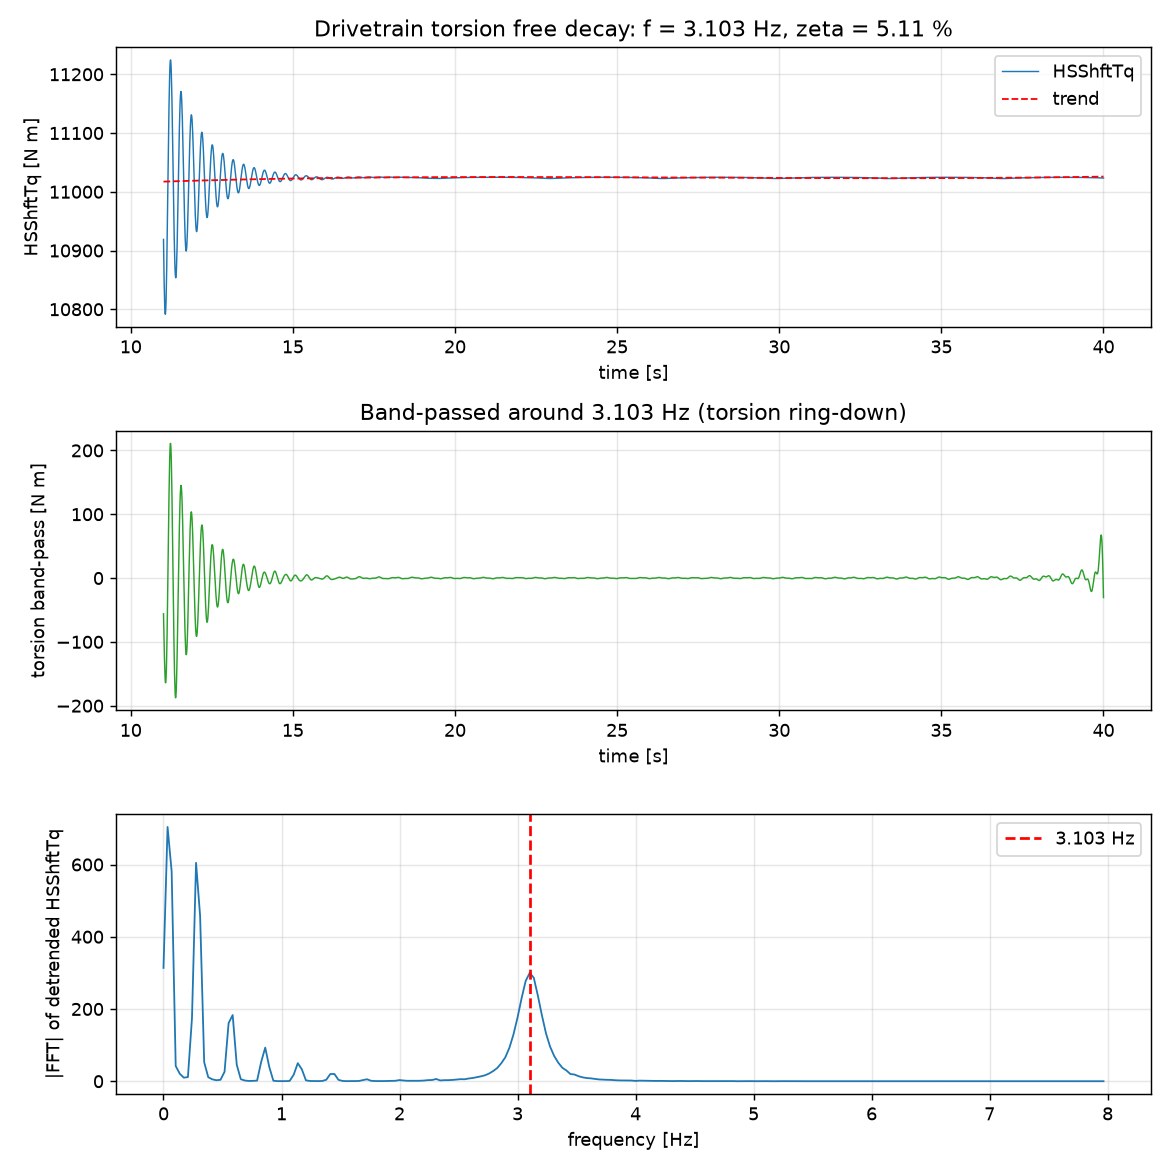
\includegraphics[width=0.85\linewidth]{fig/torsion_decay.png}
  \caption{Free-decay identification of the drivetrain torsional mode from the
  high-speed-shaft torque \texttt{HSShftTq}. \emph{Top:} raw signal and removed
  cubic trend after the \(+\SI{10}{\percent}\) torque pulse at
  \(t=\SI{10}{\second}\). \emph{Middle:} the residual band-passed around the
  torsional peak, showing a clean ring-down that decays within
  \(\approx\SI{4}{\second}\). \emph{Bottom:} FFT of the detrended residual, with
  an isolated peak at \SI{3.10}{\hertz} (dashed line) well separated from the
  sub-\SI{1}{\hertz} tower/rotor content. The fitted decay corresponds to
  \(\zeta=\SI{5.1}{\percent}\).}
  \label{fig:tors-decay}
\end{figure}

\subsection{Torque path and the ROSCO constraint}
\label{subsec:tors-torque-path}

As in \S\ref{subsec:ss-torque-path}, the electrical\(\to\)mechanical path into
the OpenFAST structure is not open by default: ROSCO (\texttt{VSContrl}=5) owns
the generator torque and rejects the external commands (\texttt{GenSpdOrTrq},
\texttt{ElecPwrCom}) crossing the FMU interface. The only channel that reaches
the structural solver is the ROSCO open-loop generator-torque table
(\texttt{OL\_Mode}=1, \texttt{Ind\_GenTq}=2). The torsional disturbance is
therefore prescribed through that table as a sinusoidal modulation about
\(T_0\), identical in form to Eq.~\eqref{eq:ss-forcing},
\begin{equation}
  T_{\mathrm{gen}}(t) = T_0\,\big[\,1 + a\,
    \sin\!\big(2\pi f\,(t-t_{\mathrm{on}})\big)\,\big]\,
    \mathbb{1}[t \ge t_{\mathrm{on}}],
  \qquad a = 0.10,\; t_{\mathrm{on}}=\SI{10}{\second}.
  \label{eq:tors-forcing}
\end{equation}
The same caveat applies: the torque source is \emph{imposed} rather than the
product of a closed grid\(\to\)torque feedback, which ROSCO blocks in this FMU
build. What the sweep establishes is the genuine OpenFAST structural physics ---
the frequency selectivity with which the drivetrain amplifies a generator-torque
oscillation.

\subsection{Sweep method}
\label{subsec:tors-method}

For each probe frequency \(f\) the coupled LEOGO\,+\,OpenFAST-FMU co-simulation
is run for \SI{30}{\second} with a fixed communication step of
\SI{0.01}{\second} and no grid load event, so the sinusoidal generator torque of
Eq.~\eqref{eq:tors-forcing} is the only disturbance. The shorter horizon than
the tower sweep is adequate because the torsional mode settles quickly: its
envelope time constant is \(\tau = 1/(\zeta\omega)\approx\SI{1}{\second}\). The
response is read from \texttt{HSShftTq}, and a sinusoid at \(f\) is fitted by
least squares over the settled window \(t\in[15,30]\,\si{\second}\),
\begin{equation}
  y(t) \approx \alpha\sin(2\pi f t) + \beta\cos(2\pi f t) + \gamma,
  \qquad
  A_{\mathrm{tor}} = \sqrt{\alpha^2 + \beta^2},
  \label{eq:tors-fit}
\end{equation}
with the fitted amplitude \(A_{\mathrm{tor}}\) as the response metric. The
sweep, table and figure are produced by
\texttt{casestudies/dyn\_sim/sweep\_torsion.py}.

\subsection{Results}
\label{subsec:tors-results}

The sweep traces out a sharp, symmetric resonance centred exactly on the
identified torsional frequency (Table~\ref{tab:tors-sweep},
Figure~\ref{fig:tors-curve}). The fitted high-speed-shaft-torque amplitude rises
from \(A_{\mathrm{tor}}\approx\SI{3.5}{\kilo\newton\metre}\) at
\SI{2.6}{\hertz} to a peak of
\(A_{\mathrm{tor}}\approx\SI{11.0}{\kilo\newton\metre}\) at \SI{3.10}{\hertz},
then falls symmetrically to \(\approx\SI{2.2}{\kilo\newton\metre}\) at
\SI{3.8}{\hertz}. The peak coincides with \(f_{\mathrm{tor}}\) from the
independent free-decay test. From the half-power bandwidth
(\(A_{\mathrm{tor}} \ge A_{\mathrm{peak}}/\sqrt2 \approx
\SI{7.8}{\kilo\newton\metre}\), spanning \(\approx\SIrange{2.94}{3.26}{\hertz}\))
the quality factor is
\begin{equation}
  Q = \frac{f_{\mathrm{tor}}}{\Delta f} \approx \frac{3.10}{0.32} \approx 9.7,
  \qquad
  \zeta = \frac{1}{2Q} \approx \SI{5.1}{\percent},
  \label{eq:tors-Q}
\end{equation}
in agreement with both the free-decay estimate of
Eq.~\eqref{eq:tors-identified} and the prescribed value of
Eq.~\eqref{eq:tors-damp}. The two independent methods --- ring-down and swept
steady-state --- thus give the same damping, a strong internal consistency
check.

Unlike the tower sweep, the torsion curve does not fall to a near-zero floor
away from resonance. This is expected and physically correct: the imposed
\(\pm\SI{10}{\percent}\) generator-torque ripple is transmitted \emph{directly}
through the shaft even off resonance, setting a non-zero baseline of order
\SIrange{2}{4}{\kilo\newton\metre}, on top of which the resonant amplification
appears as the peak. The peak-to-baseline amplification is therefore a factor of
\(\approx 3\)--\(5\).

\begin{table}[t]
  \centering
  \caption{OpenFAST-FMU frequency sweep of the drivetrain torsional response:
  least-squares fitted amplitude of \texttt{HSShftTq} at the forcing frequency
  (\(\pm\SI{10}{\percent}\) generator-torque modulation, Region~2). The bold row
  marks the identified torsional mode.}
  \label{tab:tors-sweep}
  \begin{tabular}{lc}
    \toprule
    \(f\) [\si{\hertz}] &
      \(A_{\mathrm{tor}}\) [\si{\kilo\newton\metre}] \\
    \midrule
    2.60          & 3.52 \\
    2.80          & 5.25 \\
    2.90          & 6.87 \\
    3.00          & 9.29 \\
    3.05          & 10.50 \\
    \textbf{3.10} & \textbf{11.05} \\
    3.15          & 10.54 \\
    3.20          & 9.30 \\
    3.30          & 6.67 \\
    3.50          & 3.80 \\
    3.80          & 2.17 \\
    \bottomrule
  \end{tabular}
\end{table}

\begin{figure}[t]
  \centering
  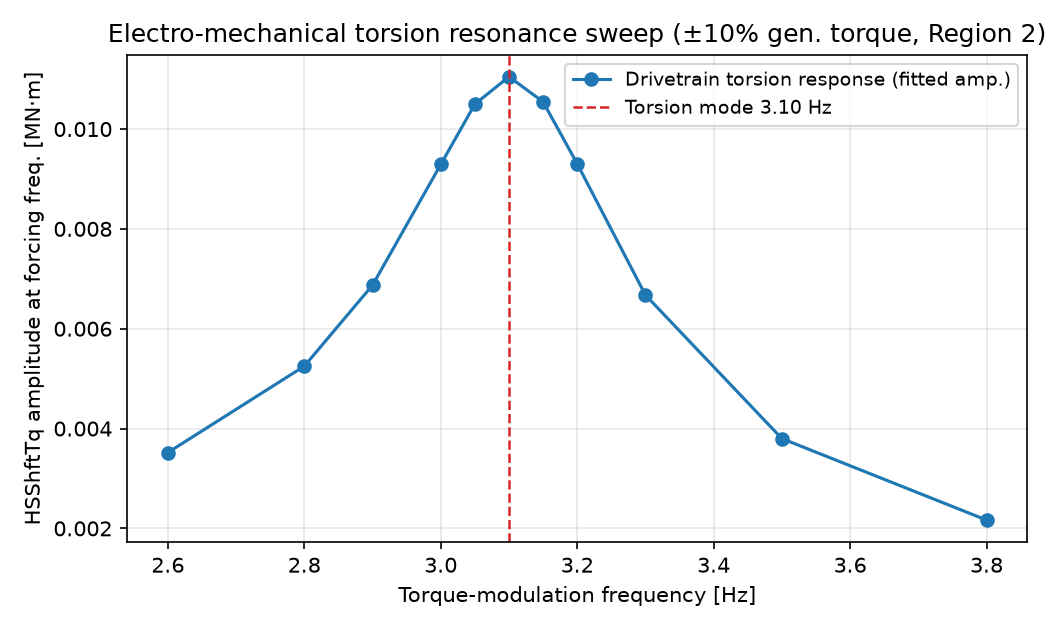
\includegraphics[width=0.8\linewidth]{fig/torsion_curve.png}
  \caption{OpenFAST-FMU model: fitted high-speed-shaft-torque amplitude
  (\texttt{HSShftTq}) versus generator-torque modulation frequency
  (\(\pm\SI{10}{\percent}\), Region~2). The response peaks sharply at the
  drivetrain torsional mode (dashed line, \SI{3.10}{\hertz}), with a
  half-power bandwidth giving \(Q\approx 9.7\) (\(\zeta\approx\SI{5.1}{\percent}\)).
  The non-zero off-resonance baseline is the imposed torque ripple transmitted
  directly through the shaft.}
  \label{fig:tors-curve}
\end{figure}

\subsection{Discussion}
\label{subsec:tors-discussion}

The drivetrain torsional sweep provides a second, mechanically independent
instance of frequency-selective electro-mechanical coupling in the high-fidelity
model. The generator-torque oscillation is amplified into a resonant shaft-torque
response only when its frequency matches the torsional eigenmode at
\SI{3.10}{\hertz}, and the resonance is narrow (\(Q\approx 10\)). Two independent
identifications --- the free-decay ring-down of \S\ref{subsec:tors-decay} and the
swept steady-state response of \S\ref{subsec:tors-results} --- agree on both the
frequency (\SI{3.10}{\hertz}) and the damping (\(\zeta\approx\SI{5.1}{\percent}\)),
and both recover the prescribed model damping of Eq.~\eqref{eq:tors-damp}.

The same two caveats as in \S\ref{subsec:ss-discussion} apply. First, the torque
is injected through the ROSCO open-loop table because the controller blocks the
genuine grid\(\to\)torque path in this FMU build; the resonant amplification is
real structural physics, but the excitation is prescribed. Second, the softened
shaft stiffness and the reduced damping are deliberate modelling choices that
move the mode into the OpenFAST bandwidth and let it ring; the frequency and
\(Q\) reported here are properties of that configured model, not of the
as-delivered IEA \SI{15}{\mega\watt} drivetrain. With these qualifications, the
result complements the tower side-to-side study: together they show that the
generator-torque channel couples selectively to two distinct lightly damped
mechanical modes --- a lateral tower mode near the LEOGO grid electromechanical
band, and a drivetrain torsional mode an order of magnitude higher --- while the
genuinely open electromagnetic-torque path is demonstrated in the reduced-model
study of \S\ref{sec:forcedresponse}.
